\documentclass[conference]{IEEEtran}
\IEEEoverridecommandlockouts

%\usepackage[a4paper, margin=1in]{geometry}
\usepackage{graphicx}
\usepackage{caption}
\usepackage{amsmath}
\usepackage{booktabs}
\usepackage{hyperref}
\usepackage{authblk}
\usepackage{tikz}
\usepackage{subcaption}
\usetikzlibrary{shapes.geometric, arrows.meta, positioning}

\tikzstyle{block} = [rectangle, draw, rounded corners, minimum height=2em, minimum width=6em, align=center]
\tikzstyle{arrow} = [-{Latex[length=3mm]}, thick]

\def\BibTeX{{\rm B\kern-.05em{\sc i\kern-.025em b}\kern-.08em
    T\kern-.1667em\lower.7ex\hbox{E}\kern-.125emX}}

\begin{document}

\title{\textbf{Investigating Frame Size Effects on Mental State Classification\\ from the Androids Corpus}}


\author{Vadim Sokolov}
\affil{Department of Computer Science, University of Milan, Milan, Italy}
\date{}

\maketitle

\begin{abstract}
Mental state detection from speech is an important task in clinical cases, that can support early diagnosis and monitoring. 
In this work, we investigate how varying frame sizes affect the accuracy of mental state prediction using audio from the Androids Corpus. 
We extract standard acoustic features (MFCCs, deltas, RMS) with varying temporal windows and evaluate performance using linear model, Random Forest and SVM, confirming the hypothesis that mental states vary slowly. 
We augmented the feature set with additional acoustic descriptors. 
Results show that nonlinear models achieve higher accuracy than the linear baseline, with the best performance exceeding 80\% when using longer frame sizes (5–10 seconds). 
The added features improved SVM performance in specific configurations but did not benefit all models. 
These findings highlight the interaction between model choice, feature selection, and temporal resolution in speech based mental state detection.

\end{abstract}

\section{Introduction}
Mental health disorders such as depression affect millions of people worldwide. 
Automatic detection of such conditions from speech gives a non invasive, scalable, and cost-effective screening mechanism. 
Speech contains both linguistic and paralinguistic features that can correlate with psychological states.

In this study, our goal is to explore how temporal framing in audio feature extraction affects classification performance. 
The assumption is that mental states change slowly over time, and thus longer frames might capture more relevant descriptors.

\section{Related Work and Motivation}
Previous work on the Androids Corpus \cite{androids2021} uses features extracted with OpenSMILE and evaluates classifiers using a speaker-independent 5-fold protocol. 
Other studies utilized deep learning, but often does not take into consideration the temporal resolution of acoustic features.

Our goal is to explore different frame lengths to understand how temporal granularity affects classification. 
We hypothesize that longer frames improve performance by capturing more stable features.

\section{Methodology}

The diagram of the method used is shown in Figure~\ref{fig:block-diagram}.
The audio recordings were resampled to 16 kHz and converted to mono. 
Frame-based feature extraction was performed using window sizes of 20 ms to 30 s, with a 50\% overlap. 
For each frame, the following features were extracted:

MFCCs (13 coefficients) capture the spectral shape of the signal.
Delta and Delta-Delta MFCCs (13 each) represent temporal dynamics.
Root Mean Square (RMS) energy measures signal power.
Fundamental frequency (F0) is estimated using \texttt{librosa.yin} \cite{librosa} for pitch-related information.
Harmonic Ratio is calculated as the ratio between harmonic and total energy via Harmonic-Percussive Source Separation (HPSS).
Each audio file was converted to a sequence of feature vectors (frames), with an optional aggregation step (mean) or majority voting used later for classification.

For the SVM classifier, an RBF kernel was used. The model was implemented using the Scikit-learn library \cite{sklearn}.
Initial hyperparameters were obtained via a combination of grid search and manual tuning: C = 0.3, $\gamma = 0.01$, and class weights {0: 1.0, 1: 0.8}. 
These served as the baseline parameters for experiments prior to adding new features.

\subsection{Dataset}
We use the Androids Corpus, which contains recordings from interviews and reading tasks by individuals classified as either healthy controls or patients.
\begin{table}[h]
\centering
\caption{Summary of the Androids Corpus structure and contents.}
\resizebox{\linewidth}{!}{
%\begin{tabular}{p{4.2cm} p{8cm}}
\begin{tabular}{|c|c|}
\hline
\textbf{Component} & \textbf{Description} \\
\hline
\texttt{Reading-Task/} & 112 audio recordings of participants reading a fairy tale. \\
    & Subfolders: \texttt{HC/} (54 files) and \texttt{PT/} (58 files). \\
\hline
\texttt{Interview-Task/audio/} & 116 full interview recordings. \\
    & Subfolders: \texttt{HC/} (52 files) and \texttt{PT/} (64 files). \\
\hline
\texttt{Interview-Task/} \newline \texttt{audio\_clip/} & 874 segmented audio clips from interviews, \\
    & distributed over 116 subdirectories (one per speaker). \\
\hline
\texttt{Labels} & Each file is labeled by condition: \texttt{PT} (patient) or \texttt{C} (control). \\
\hline
\texttt{Naming convention} & \texttt{nn\_XGmm\_t.wav}, where fields encode speaker ID, \\
    & condition, gender, age, and education level. \\
\hline
\end{tabular}
}
%\caption{Summary of the Androids Corpus structure and contents.}
\label{tab:androids_summary}
\end{table}

\begin{figure*}[ht]
\begin{center}
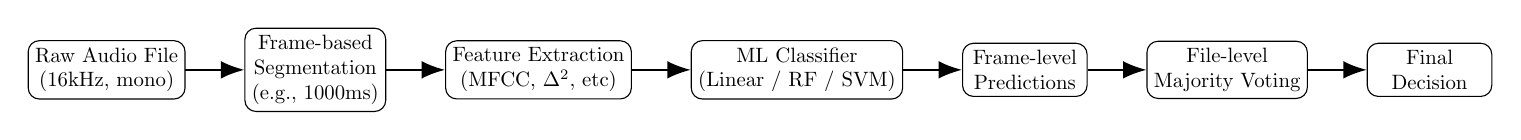
\begin{tikzpicture}[node distance=1.8cm and 1cm, scale=0.75, transform shape]

\node[block] (audio) {Raw Audio File\\(16kHz, mono)};
\node[block, right=of audio] (frames) {Frame-based\\Segmentation\\(e.g., 1000ms)};
\node[block, right=of frames] (features) {Feature Extraction\\(MFCC, $\Delta^2$, etc)};
\node[block, right=of features] (ml) {ML Classifier\\(Linear / RF / SVM)};
\node[block, right=of ml] (framepred) {Frame-level\\Predictions};
\node[block, right=of framepred] (vote) {File-level\\Majority Voting};
\node[block, right=of vote] (final) {Final\\Decision};

\draw[arrow] (audio) -- (frames);
\draw[arrow] (frames) -- (features);
\draw[arrow] (features) -- (ml);
\draw[arrow] (ml) -- (framepred);
\draw[arrow] (framepred) -- (vote);
\draw[arrow] (vote) -- (final);

\end{tikzpicture}
\caption{Overview of the proposed processing pipeline.}
\label{fig:block-diagram}
\end{center}
\end{figure*}


\subsection{Feature Extraction}
We extract the following features using \texttt{librosa}:
\begin{itemize}
    \item 13 MFCCs
    \item Delta and Delta-Delta of MFCCs
    \item Root Mean Square (RMS) Energy
\end{itemize}

We experiment with different frame sizes: 20ms, 30ms, 100ms, 250ms, 500ms, 1000ms, 5000ms, and 10000ms. 
We study 20s and 30s frame sizes to make sure the patterns no longer persist with drastically wide windows. 
All features are normalized using standard scaling.
The dataset was filtered so no speaker appears in both train and test sets.

\subsection{Classification}
We start with a logistic regression model and evaluate frame-level accuracy and F1 score. 
The dataset is split using a speaker-independent 5-fold division, consistent with the original baseline setup, which can be seen at Table~\ref{tab:androids_summary}.
Implemented file-level majority voting like a BS2 baseline in the original paper.
Compared frame level against file level performance.
Different models (Linear, RF, SVM) were tested separately and compared using speaker independent 5-fold cross-validation 
to perform depression vs. control classification at the frame level.

\subsection{PCA analysis}

Principal Component Analysis (PCA) was applied after feature standardization to address the curse of dimensionality. 
PCA was fitted on the training set and applied to both training and test sets. It retained the minimum number of components to keep at least 95\% of the variance. 
This step was repeated for each frame size and the testing model to provide adaptation to the specific data distribution.

\section{Experiments and Results}

\subsection{Evaluation Metrics}
For frame level evaluation the following metrics were used:
\begin{itemize}
    \item Frame-level accuracy
    \item Frame-level F1 score
    \item Confusion matrix (TBD)
\end{itemize}

For file level evaluation the majority voting was used to align with BS2 baseline, improve robustness.

\subsection{Results}

\begin{figure}[h]
    \centering
    \includegraphics[width=\linewidth]{../out/modelPerfvsFrameSize.png}
    \caption{Accuracy and F1 Score vs Frame Size (log-scale)}
    \label{fig:model_perf}
\end{figure}

Initial results show that performance improves with larger frame sizes, peaking around 10000–20000ms.
At the plots \ref{fig:model_perf} one can see the comparison between different classifiers: Logistic regression, Random Forest, and SVM.
One can see precise results in a Table~\ref{tab:linear_model_perf}, Table~\ref{tab:random_forest_perf}, and Table~\ref{tab:svm_perf}.

\subsection{Feature importance analysis}

\begin{figure}[h]
    \centering
    \includegraphics[width=\linewidth]{../out/feature_imp_1000ms.png}
    \caption{Feature importances from Random Forest model.}
    \label{fig:feature_importance}
\end{figure}

After the performance comparison it was decided to analyze the feature importance and possibly add some more of them to the models.
The feature importance analysis was conducted to a Random Forest model. 
It is shown as an example in Figure~\ref{fig:feature_importance} for the frame size of 1000ms.

The top features were identified as follows: mmcf\_2, mfcc\_1, and RMS. 
These features were not consistent across all frame sizes. 
The statistics changed for larger frame sizes, where other features like mfcc\_13 appeared.

\subsection{Performance of the classifiers with added features}

\begin{figure}[h]
    \centering
    \includegraphics[width=\linewidth]{../out/modelPerfvsFrameSizeAdded.png}
    \caption{Accuracy and F1 Score with added features vs Frame Size (log-scale)}
    \label{fig:model_perf_added}
\end{figure}

We added more features to the models, such as fundamental frequency (F0) and harmonic ratio, to see if they improve performance.
The model performance can be seen on Table~\ref{tab:linear_model_added_feat_perf}, Table~\ref{tab:random_forest_added_feat_perf}, and Table~\ref{tab:svm_added_feat_perf}.


% \begin{figure}[ht]
%     \centering
%     \includegraphics[width=0.48\textwidth]{../out/lr_cm_file_level.png}
%     \caption{Confusion matrix (\%) for file-level classification using Random Forest, frame size = 10s.}
%     \label{fig:cm_lr_10s}
% \end{figure}

\begin{figure}[ht]
    \centering
    \captionsetup{font=small}
    \begin{subfigure}[b]{0.23\textwidth}
        \centering
        \includegraphics[width=\textwidth]{../out/rf_cm_file_level_10000ms.png}
        \caption{Random Forest, frame size = 10s}
        \label{fig:cm_rf_10s}
    \end{subfigure}
    \hfill
    \begin{subfigure}[b]{0.23\textwidth}
        \centering
        \includegraphics[width=\textwidth]{../out/svm_cm_file_level_5000ms.png}
        \caption{SVM, frame size = 5s}
        \label{fig:cm_svm_5s}
    \end{subfigure}
    \caption{Confusion matrices (\%) for file-level classification.}
    \label{fig:cm_comparison}
\end{figure}

Figure \ref{fig:cm_comparison} shows the file-level confusion matrices (in \%) for the best-performing configurations of SVM and Random Forest.
The model correctly classified 62.21\% of class 0 samples and 19.19\% of class 1 samples, with most misclassifications coming from class 1 being labeled as class 0 (13.37\%).
Random forest model achieved a more balanced performance between classes, with a lower false negative rate compared to SVM.

% Linear model

\begin{table}[h]
\centering
\caption{Linear model performance.}
\begin{tabular}{|c|c|c|}
\hline
\textbf{Frame size, ms} & \textbf{Accuracy} & \textbf{F1-score}\\
\hline
20 & 0.6455 & 0.6278 \\
\hline
30 & 0.6506 & 0.6296 \\
\hline
100 & 0.6635 & 0.6337 \\
\hline
250 & 0.6583 & 0.6269 \\
\hline
500 & 0.6640 & 0.6300 \\
\hline
1000 & 0.6684 & 0.6296 \\
\hline
5000 & 0.7067 & 0.5829 \\
\hline
10000 & 0.7255 & 0.6400 \\
\hline
15000 & 0.7290 & 0.6849 \\
\hline
20000 & 0.7317 & 0.6786 \\
\hline
30000 & 0.7074 & 0.7074 \\
\hline
\end{tabular}
\label{tab:linear_model_perf}
\end{table}

% Random forest

\begin{table}[h]
\centering
\caption{Random forest performance.}
\begin{tabular}{|c|c|c|}
\hline
\textbf{Frame size, ms} & \textbf{Accuracy} & \textbf{F1-score}\\
\hline
20 & 0.6799 & 0.6115 \\
\hline
30 & 0.6829 & 0.6115 \\
\hline
100 & 0.6788 & 0.6027 \\
\hline
250 & 0.6661 & 0.5907 \\
\hline
500 & 0.6618 & 0.5945 \\
\hline
1000 & 0.6589 & 0.5957 \\
\hline
5000 & 0.6693 & 0.5799 \\
\hline
10000 & 0.6894 & 0.6006 \\
\hline
15000 & 0.6898 & 0.6398 \\
\hline
20000 & 0.6477 & 0.5925 \\
\hline
30000 & 0.6352 & 0.5873 \\
\hline
\end{tabular}
\label{tab:random_forest_perf}
\end{table}

% SVM

\begin{table}[h]
\centering
\caption{SVM performance.}
\begin{tabular}{|c|c|c|}
\hline
\textbf{Frame size, ms} & \textbf{Accuracy} & \textbf{F1-score}\\
\hline
20 & 0.6635 & 0.5833 \\
\hline
30 & 0.6736 & 0.5908 \\
\hline
100 & 0.6824 & 0.5976 \\
\hline
250 & 0.6996 & 0.6053 \\
\hline
500 & 0.6890 & 0.5854 \\
\hline
1000 & 0.6916 & 0.5823 \\
\hline
5000 & 0.7186 & 0.5217 \\
\hline
10000 & 0.7576 & 0.6196 \\
\hline
15000 & 0.7245 & 0.6455 \\
\hline
20000 & 0.7575 & 0.6427 \\
\hline
30000 & 0.7556 & 0.7054 \\
\hline
\end{tabular}
\label{tab:svm_perf}
\end{table}

\subsection{PCA analysis}
PCA analysis is used to reduce the number of features and therefore address the curse of dimensionality. 
We are preserving 95\% of variance to transform the dataset and get less uncorrelated "principal components" that preserve most of the variance.
For example, instead of 42 extended features we got 34-37 features.
We used 1000ms, 5000ms, 10000ms, 15000ms frames to study the effect of PCA on accuracy.
The tables \ref{tab:linear_model_pca}, \ref{tab:random_forest_pca}, and \ref{tab:svm_pca} represent classifiers performance with PCA reduced features.

\section{Discussion}
Larger frames provide better performance, suggesting that mental state-related features are better captured over longer time spans. 
Short frames likely introduce variability and noise.

\subsection{Feature importance analysis}

Directly extracted and visualized feature importances. 
As a result, one can see that RMS is among the top features. 
That could indicate energy is a good mental state marker.

\begin{table}[h]
\centering
\caption{Feature importance analysis.}
\begin{tabular}{|c|c|c|c|}
\hline
\textbf{Frame size, ms} & \textbf{Top Feature} & \textbf{2nd Feature} & \textbf{3rd Feature}\\
\hline
20 & mfcc\_2 & mfcc\_1 & rms \\
\hline
30 & mfcc\_2 & mfcc\_1 & rms \\
\hline
100 & mfcc\_2 & mfcc\_1 & rms \\
\hline
250 & mfcc\_2 & mfcc\_1 & rms \\
\hline
500 & mfcc\_1 & mfcc\_2 & rms \\
\hline
1000 & mfcc\_1 & mfcc\_2 & rms \\
\hline
5000 & mfcc\_2 & mfcc\_1 & rms \\
\hline
10000 & mfcc\_2 & mfcc\_1 & rms \\
\hline
15000 & mfcc\_1 & mfcc\_2 & rms \\
\hline
20000 & mfcc\_2 & mfcc\_1 & mfcc\_13 \\
\hline
30000 & mfcc\_2 & mfcc\_1 & mfcc\_6 \\
\hline
\end{tabular}
\label{tab:feaure_importance}
\end{table}


From the Table~\ref{tab:feaure_importance} one can see that the RMS moves from top 3 features to 4th place for the frame size 20s and 30s.
When we compute feature importances from a Random Forest using \texttt{.feature\_importances\_}, what we're actually getting is the Mean Decrease in Impurity (MDI). 
Impurity refers to how mixed the class labels are in a node.
Higher MDI equals to a fact that feature was used more often and split more samples while significantly reducing impurity thus, 
more important.


\subsection{Performance of the classifiers with added features}

% linear

\begin{table}[h]
\centering
\caption{Linear model performance with added features.}
\resizebox{\linewidth}{!}{
\begin{tabular}{|c|c|c|c|c|}
\hline
\textbf{Frame size, ms} & \textbf{Frame-level Accuracy} & \textbf{Frame-level F1-score} & \textbf{File-level Accuracy} & \textbf{File-level F1-score} \\
\hline
20 & 0.6695 & 0.6248 & 0.7415 & 0.6433 \\
\hline
30 & 0.6718 & 0.6257 & 0.7542 & 0.6667 \\
\hline
100 & 0.6820 & 0.6318 & 0.7669 & 0.6746 \\
\hline
250 & 0.6746 & 0.6225 & 0.7627 & 0.6627 \\
\hline
500 & 0.6767 & 0.6245 & 0.7350 & 0.6310 \\
\hline
1000 & 0.6895 & 0.6356 & 0.7301 & 0.6164 \\
\hline
5000 & 0.7272 & 0.6756 & 0.7791 & 0.6885 \\
\hline
10000 & 0.7274 & 0.6721 & 0.7630 & 0.6444 \\
\hline
15000 & 0.7428 & 0.7138 & 0.7071 & 0.6420 \\
\hline
20000 & 0.6877 & 0.6489 & 0.6463 & 0.5672 \\
\hline
30000 & 0.7133 & 0.6993 & 0.7167 & 0.6909 \\
\hline
\end{tabular}
}
\label{tab:linear_model_added_feat_perf}
\end{table}

% random forest

File-level accuracy was evaluated as well. It was estimated by majority voting as in bs2 baseline.
F1 score for random forest is remarkably high in file level estimation, reaching 0.79 fir 30s frames (see Figure~\ref{fig:model_perf_added}).

\begin{table}[h]
\centering
\caption{Random forest performance with added features.}
\resizebox{\linewidth}{!}{
\begin{tabular}{|c|c|c|c|c|}
\hline
\textbf{Frame size, ms} & \textbf{Frame-level Accuracy} & \textbf{Frame-level F1-score} & \textbf{File-level Accuracy} & \textbf{File-level F1-score} \\
\hline
20 & 0.6820 & 0.6290 & 0.7966 & 0.6923 \\
\hline
30 & 0.6849 & 0.6281 & 0.7966 & 0.6883 \\
\hline
100 & 0.6813 & 0.6224 & 0.7839 & 0.6752 \\
\hline
250 & 0.6703 & 0.6130 & 0.7585 & 0.6460 \\
\hline
500 & 0.6684 & 0.6144 & 0.7393 & 0.6303 \\
\hline
1000 & 0.6715 & 0.6272 & 0.7168 & 0.6279 \\
\hline
5000 & 0.7437 & 0.7087 & 0.8023 & 0.7302 \\
\hline
10000 & 0.7495 & 0.7162 & 0.8148 & 0.7475 \\
\hline
15000 & 0.7399 & 0.7239 & 0.7576 & 0.7000 \\
\hline
20000 & 0.6957 & 0.6883 & 0.7317 & 0.7027 \\
\hline
30000 & 0.7733 & 0.7792 & 0.8000 & 0.7931 \\
\hline
\end{tabular}
}
\label{tab:random_forest_added_feat_perf}
\end{table}

% svm

\begin{table}[h]
\centering
\caption{SVM performance with added features.}
\resizebox{\linewidth}{!}{
\begin{tabular}{|c|c|c|c|c|}
\hline
\textbf{Frame size, ms} & \textbf{Frame-level Accuracy} & \textbf{Frame-level F1-score} & \textbf{File-level Accuracy} & \textbf{File-level F1-score} \\
\hline
20 & 0.6774 & 0.5848 & 0.7873 & 0.6694 \\
\hline
30 & 0.6849 & 0.6022 & 0.7992 & 0.6749 \\
\hline
100 & 0.7169 & 0.6154 & 0.8263 & 0.6963 \\
\hline
250 & 0.7044 & 0.5912 & 0.8263 & 0.6822 \\
\hline
500 & 0.6893 & 0.5662 & 0.7949 & 0.6190 \\
\hline
1000 & 0.6903 & 0.5646 & 0.7876 & 0.6000 \\
\hline
5000 & 0.7465 & 0.6573 & 0.8140 & 0.6735 \\
\hline
10000 & 0.7495 & 0.6790 & 0.8000 & 0.6897 \\
\hline
15000 & 0.7428 & 0.6942 & 0.7273 & 0.6494 \\
\hline
20000 & 0.7589 & 0.6806 & 0.7317 & 0.6071 \\
\hline
30000 & 0.7333 & 0.7059 & 0.7333 & 0.7037 \\
\hline
\end{tabular}
}
\label{tab:svm_added_feat_perf}
\end{table}

\subsection{PCA analysis}

% linear

\begin{table}[h]
\centering
\caption{Linear model performance with PCA-reduced features.}
\resizebox{\linewidth}{!}{
\begin{tabular}{|c|c|c|c|c|c|}
\hline
\textbf{Frame size, ms} & \textbf{PCA} & \textbf{Frame-level Accuracy} & \textbf{Frame-level F1-score} & \textbf{File-level Accuracy} & \textbf{File-level F1-score} \\
\hline
1000 & no & 0.6895 & 0.6356 & 0.7301 & 0.6164 \\
\hline
1000 & yes & 0.6712 & 0.6131 & 0.7522 & 0.6410 \\
\hline
5000 & no & 0.7272 & 0.6756 & 0.7791 & 0.6885 \\
\hline
5000 & yes & 0.7272 & 0.6767 & 0.7674 & 0.6774 \\
\hline
10000 & no & 0.7274 & 0.6721 & 0.7630 & 0.6444 \\
\hline
10000 & yes & 0.7216 & 0.6734 & 0.7556 & 0.6667 \\
\hline
15000 & no & 0.7428 & 0.7138 & 0.7071 & 0.6420 \\
\hline
15000 & yes & 0.7312 & 0.7138 & 0.6869 & 0.6517 \\
\hline
\end{tabular}
}
\label{tab:linear_model_pca}
\end{table}


PCA for linear classifier gives slightly worse results than without PCA.
There are several reasons why PCA hurts linear model performance. 
First, PCA is unsupervised, it preserves the variance and doesn't preserve the separation of classes.
It can remove important discriminative information for the classifier.
Second, the used features may already be informative, good in separating classes.
PCA might delute their effects. 

% Random forest

\begin{table}[h]
\centering
\caption{Random Forest performance with PCA-reduced features.}
\resizebox{\linewidth}{!}{
\begin{tabular}{|c|c|c|c|c|c|}
\hline
\textbf{Frame size, ms} & \textbf{PCA} & \textbf{Frame-level Accuracy} & \textbf{Frame-level F1-score} & \textbf{File-level Accuracy} & \textbf{File-level F1-score} \\
\hline
1000 & no & 0.6715 & 0.6272 & 0.7168 & 0.6279 \\
\hline
1000 & yes & 0.6521 & 0.6050 & 0.7434 & 0.6375 \\
\hline
5000 & no & 0.7437 & 0.7087 & 0.8023 & 0.7302 \\
\hline
5000 & yes & 0.7375 & 0.6934 & 0.8256 & 0.7458 \\
\hline
10000 & no & 0.7495 & 0.7162 & 0.8148 & 0.7475 \\
\hline
10000 & yes & 0.7283 & 0.6981 & 0.7704 & 0.6931 \\
\hline
15000 & no & 0.7399 & 0.7239 & 0.7576 & 0.7000 \\
\hline
15000 & yes & 0.6965 & 0.6749 & 0.6869 & 0.6353 \\
\hline
\end{tabular}
}
\label{tab:random_forest_pca}
\end{table}

% svm

\begin{table}[h]
\centering
\caption{SVM performance with PCA-reduced features.}
\resizebox{\linewidth}{!}{
\begin{tabular}{|c|c|c|c|c|c|}
\hline
\textbf{Frame size, ms} & \textbf{PCA} & \textbf{Frame-level Accuracy} & \textbf{Frame-level F1-score} & \textbf{File-level Accuracy} & \textbf{File-level F1-score} \\
\hline
1000 & no & 0.6903 & 0.5646 & 0.7876 & 0.6000 \\
\hline
1000 & yes & 0.6801 & 0.5669 & 0.7522 & 0.5692 \\
\hline
5000 & no & 0.7465 & 0.6573 & 0.8140 & 0.6735 \\
\hline
5000 & yes & 0.7484 & 0.6679 & 0.8256 & 0.7222 \\
\hline
10000 & no & 0.7495 & 0.6790 & 0.8000 & 0.6897 \\
\hline
10000 & yes & 0.7399 & 0.6723 & 0.7704 & 0.6437 \\
\hline
15000 & no & 0.7428 & 0.6942 & 0.7273 & 0.6494 \\
\hline
15000 & yes & 0.7399 & 0.7020 & 0.7374 & 0.6750 \\
\hline
\end{tabular}
}
\label{tab:svm_pca}
\end{table}

Effect of PCA on File-level accuracy.
For linear classifier, PCA improved results only at short frame size of 1000ms.
For Random forest, PCA improved the results at shorter durations of 1000ms, 5000ms, possibly reducing overfitting.
For SVM, PCA was beneficial at medium and long frames of 5000ms, 15000ms, which is typical for high dimentional models.

To sum up, PCA is not always beneficial. 
For linear models, PCA removes useful signal unless there is strong redundancy.
For nonlinear models, PCA helps to reduce the noise and address the curse of dimensionality.

\section{Conclusion}
This paper presents an analysis of frame size on speech-based mental state classification. 
Our experiments show a consistent trend where longer frame sizes (10–20 seconds) yield higher file-level accuracy, supporting the hypothesis that slowly varying speech descriptors carry more discriminative information for this task.
We also compared models with and without additional features (fundamental frequency, harmonic ratio) and with PCA-based dimensionality reduction. 
While these features improved SVM performance in certain frame-size configurations, they did not benefit the linear model and sometimes decreased performance due to the curse of dimensionality. 
PCA occasionally improved results, particularly for Random Forest and SVM with smaller frame sizes (1–5 seconds), but generally led to lower frame-level accuracy.
The best file-level accuracy achieved was above 80\% using Random Forest (10s frames) and SVM (5s frames), with majority voting per file as in the BS2 baseline from the original dataset paper. 
These findings confirm that longer analysis windows help capture stable characteristics relevant to mental state detection while model choice and feature selection interact strongly with the optimal frame size.

\begin{thebibliography}{9}
\bibitem{androids2021}
Alessandro Vinciarelli, University of Glasgow et al. \textit{The Androids Corpus: A New Publicly Available Benchmark for Speech Based Depression Detection}. Interspeech 2023.

\bibitem{librosa}
Brian McFee et al. \textit{librosa: Audio and music signal analysis in Python}. Proceedings of the 14th python in science conference. 2015.

\bibitem{sklearn}
Pedregosa et al. \textit{Scikit-learn: Machine Learning in Python}. JMLR 2011.

\end{thebibliography}

\end{document}
